\documentclass[twoside]{amsart}
\usepackage{amssymb,latexsym}
\usepackage{amsfonts}
\usepackage{xspace}
\usepackage{enumerate}
\usepackage{graphics}
\usepackage{fitch}
\newcommand{\Rationals}{\mathbb{Q}{}}
\newcommand{\Reals}{\ensuremath{\mathbb{R}}\xspace}
\newcommand{\Integers}{\ensuremath{\mathbb{Z}{}}\xspace}
\newcommand{\solution}{\textsc{Solution}\xspace}
\newcommand{\problem}{\textsc{Problem}\xspace}
\newcommand{\Blank}{\mathrel{\phantom{=}}}
\newcommand{\ltrue}{\top}
\newcommand{\lfalse}{\bot}
\newcommand{\fOfg}{\ensuremath{f \circ g}\xspace}
\newcommand{\gOff}{\ensuremath{g \circ f}\xspace}
\newcommand{\eps}{\ensuremath{\epsilon}\xspace}
\newcommand{\iso}{\cong}
\newcommand{\niso}{\ncong}
\newcommand{\blank}{\vspace{5pt}}
\newcommand{\ind}{\hspace{.35in}}
\newcommand{\degree}{\ensuremath{^\circ}}
\newcommand{\real}{\mathop{\mathrm{real}}}
\newcommand{\img}{\mathop{\mathrm{img}}}
\newcommand{\first}{\mathop{\mathrm{first}}}
\newcommand{\second}{\mathop{\mathrm{second}}}
\newcommand{\abs}{\mathop{\mathrm{abs}}}
\begin{document}
\title{Answers to Chapter 9 Exercises - A Book of Abstract Algebra}
\author{Michael Welch}
\date{\today}
\maketitle

This document contains selected answers to exercises from chapter 9
of A Book of Abstract Algebra.


\begin{enumerate}[A.]
   \item \textsc{Isomorphism Is an Equivalence Relation among Groups}
   The following three facts about isomorphism are true for all groups:

   \blank
   \begin{enumerate}[(i)]
      \item Every group is isomorphic to itself.
      \item If $G_1 \iso G_2$, then $G_2 \iso G_1$.
      \item If $G_1 \iso G_2$ and $G_2 \iso G_3$, then $G_1 \iso G_3$.
   \end{enumerate}
   \blank

   Fact (i) asserts that for any group $G$, there exists an isomorphism 
   from $G$ to $G$.

   Fact (ii) asserts that, if there is an isomorphism $f$ from $G_1$ to
   $G_2$, there must be some isomorphism from $G_2$ to $G_1$. Well, the
   inverse of $f$ is such an isomorphism.

   Fact (iii) asserts that, if there are isomorphisms $f : G_1 \to G_2$ and
   $g : G_2 \to G_3$, there must be an isomorphism from $G_1$ to $G_3$. One can
   easily guess that $g \circ f$ is such an isomorphism. The details of
   (i), (ii), and (iii) are left as exercises.
   \blank

   \begin{enumerate}[1]
   
   \item Let $G$ be any group. If $\epsilon : G \to G$ is the identity
   function, $\epsilon(x) = x$, show that $\epsilon$ is an isomorphism.

   \blank \noindent \solution To show this, we must show that
   $\epsilon$ is a bijective function and that the property
   $\epsilon(ab)=\epsilon(a)\epsilon(b)$.

   It is injective because if $\epsilon(a)=\epsilon(b)$ then we know
   $a=b$. It is surjective because for any $y$ I know $x = [\epsilon(y)]^{-1}$
   for $x=y$. Therefore it is bijective.

   The isomorphic property is trivial to show. 
   \begin{align*}
       \epsilon(ab) &= ab && \text{Definition of identity} \\
                    &= \epsilon(a)\epsilon(b) && \text{Defn of identity twice}
   \end{align*}

   \item Let $G_1$ and $G_2$ be groups, and $f: G_1 \to G_2$ an isomorphism.
   Show that $f^{-1} : G_2 \to G_1$ is an isomorphism. [\textsc{Hint}:
   Review the discussion of inverse functions at the end of Chapter 6. Then,
   for arbitrary elements $c, d \in G_2$, there exist $a, b \in G_1$ such
   that $c = f(a)$ and $d = f(b)$. Note that $a = f^{-1}(c)$ and 
   $b = f^{-1}(d)$. Show that $f^{-1}(cd)=f^{-1}(c)f^{-1}(d)$.]

   \blank \noindent \solution Since $f$ is bijective we know that
   $f^{-1}$ is bijective. We know that $f(ab)=f(a)f(b)=cd$. Therefore
   $f^{-1}(cd)=ab=f^{-1}(c)f^{-1}(d)$. Therefore $f^{-1}$ is an isomorphism.

   \item Let $G_1$, $G_2$, and $G_3$ be groups, and let $f: G_1 \to G_2$ and
   $g:G_2 \to G_3$ be isomorphisms. Prove that $g \circ f : G_1 \to G_3$ is
   an isomorphism.

   \blank \noindent \solution The function $g \circ f$ is injective:
   Assume $(g \circ f)(a) = (g \circ f)(b)$. Then $g(f(a)) = g(f(b))$. But
   since $g$ is bijective we know that $f(a)=f(b)$. And since $f$ is
   bijective we know that $a=b$. Therefore $g \circ f$ is injective.

   \ind The function $g \circ f$ is surjective. Choose some element $y \in G_3$.
   Since $g$ is surjective we know there exist some $x \in G_2$ with
   the value $x = g^{-1}(y)$. Likewise, because $f$ is surjective
   we know there is some $z \in G_1$ with the value $z = f^{-1}(x)$. 
   Therefore $g \circ f$ is surjective and therefore it is bijective.

   Now we must show that $(g \circ f)(ab) = (g\circ f)(a)(g\circ f)(b)$.
   \begin{align}
      (g \circ f)(ab) &= g(f(ab))   \\
                      &= g(f(a)f(b))  && \text{$f$ is isomorphic (1)} \\
                      &= g(f(a)) g(f(b)) && \text{$g$ is isomorphic (2)} \\
                      &= (g \circ f)(a) (g\circ f)(b)
   \end{align}

   \end{enumerate}

   \item \textsc{Elements Which Correspond under an Isomophism}
   Recall that an isomorphism $f$ from $G_1$ to $G_2$ is a one-to-one
   correspondence between $G_1$ and $G_2$ satisfying $f(ab)=f(a)f(b)$.
   $f$ matches every element of $G_1$ with a corresponding element of
   $G_2$. It is important to note that:
   \blank

   \begin{enumerate}[(i)]
      \item $f$ matches the neutral element of $G_1$ with the neutral
      element of $G_2$.

      \item If $f$ matches an element $x$ in $G_1$ with $y$ in $G_2$,
      then, necessarily, $f$ matches $x^{-1}$ with $y^{-1}$.
      That is, if $x \leftrightarrow y$, then $x^{-1} \leftrightarrow
      y^{-1}$.

      \item $f$ matches a generator of $G_1$ with a generator of $G_2$.

      \blank
      \begin{center}
      \scalebox{1.2}{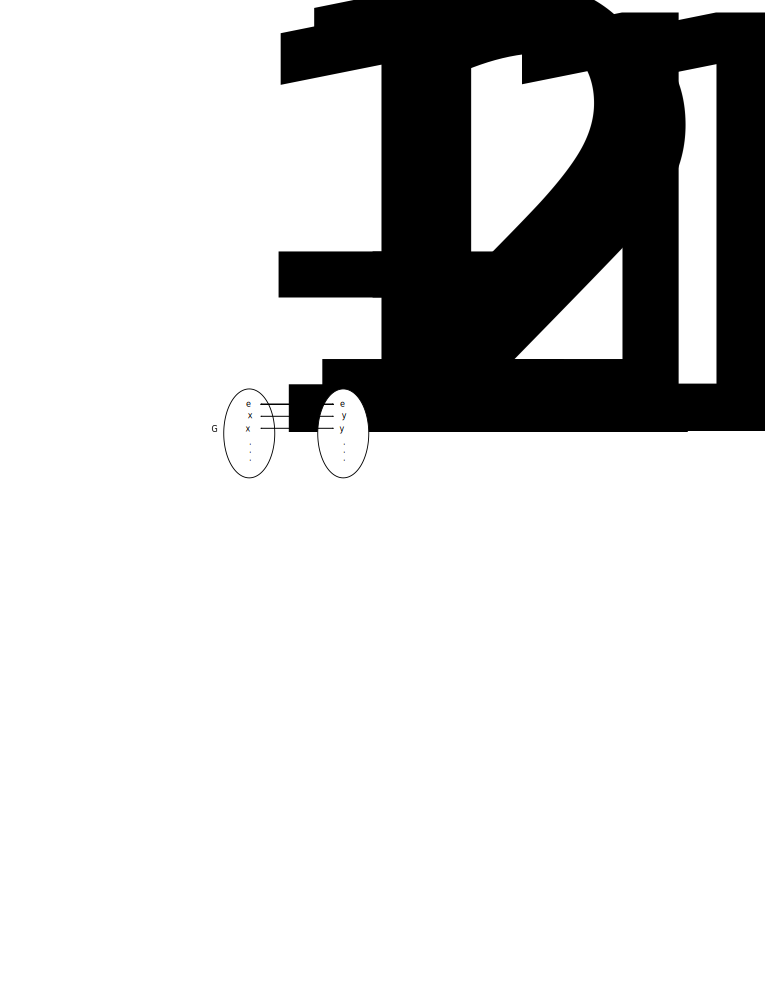
\includegraphics{img/chap9b.pdf}}
      \end{center}
      \blank

      The details of these statements are now left as an exercise. Let 
      $G_1$ and $G_2$ be groups, and let $f : G_1 \to G_2$ be an 
      isomorphism.

      \begin{enumerate}[1.]
         \item If $e_1$ deontes the neutral element of $G_1$ and $e_2$
         denotes the neutral element of $G_2$, prove that $f(e_1)=e_2$.
         [\textsc{Hint}: In any group, there is exactly one neutral
         element; show that $f(e_1)$ is the neutral element of $G_2$.]

         \setcounter{equation}{0}
         \blank \noindent \solution 
         \begin{align}
            f(ae_1) &= f(a)   && \text{Identity}\\
            f(ae_1) &= f(a)f(e_1) && \text{Isomorphism}\\
            f(a)    &= f(a)f(e_1) && \text{(1) and (2)}\\
            f(a)e_2 &= f(a)f(e_1) && \text{Identity of $e_2$}\\
                e_2 &= f(e_1)     && \text{Cancellation}
         \end{align}

         \item Prove the for each element $a$ in $G_1$, $f(a^{-1})
         = [f(a)]^{-1}$. (\textsc{Hint}: You may use Theorem 2 of 
         Chapter 4.)

         \setcounter{equation}{0}
         \blank \noindent \solution 
         \begin{align}
            f(aa^{-1}) &= f(e)          && \text{Inverses} \\
            f(aa^{-1}) &= f(a)f(a^{-1}) && \text{Isomorphism} \\
            f(e)       &= f(a)f(a^{-1}) && \text{(2) and (3)} \\
            f(a^{-1})  &= [f(a)]^{-1}   && \text{Theorem 2 of Chap 4 (3)}
         \end{align}

         \item If $G_1$ is a cyclic group with generator $a$, prove
         that $G_2$ is also a cyclic group, with generator $f(a)$.

         \blank \noindent \solution Choose any element $y \in G_2$. 
         Let $x = f^{-1}(y)$. We know that $x = a^n$ for some value of $n$.
         If $n=0$ then we have $y = f(e_1) = e_2 = [f(a)]^0$.
         If $n>0$ then $y = f(a^n) = \underbrace{f(a)f(a)\cdots f(a)}_{n
         \text{ times}} = [f(a)]^n$. Finally, if $n<0$ then
         $y = f(a^n) = \underbrace{f(a^{-1})f(a^{-1})\cdots f(a^{-1})}_{-n
         \text{ times}} = [f(a^{-1})]^{-n}$. From part 2 we know that
         $f(a^{-1}) = [f(a)]^{-1}$. Therefore 
         $[f(a^{-1})]^{-n} = ([f(a)]^{-1})^{-n}$. For each value of
         $n$ we have shown how to generate $y$ from $f(a)$. And since,
         $y$ was an arbitrary element of $G_2$ this means any element
         of $G_2$ can be generated from $f(a)$. Therefore,
         $G_2$ is a cyclic group with generator $f(a)$.

      \end{enumerate}

   \end{enumerate}

   \blank
   \item \textsc{Isomorphism of Some Finite Groups}

   In each of the following, $G$ and $H$ are finite groups. Determine whether 
   or not $G \iso H$. Prove your answer in either case.

   To find an isomorphism from $G$ to $H$ will require a little 
   ingenuity. For example, if $G$ and $H$ are cyclic groups, it is clear
   that we must match a generator $a$ of $G$ with a generator $b$ of
   $H$; that is $f(a)=b$. Then $f(aa)=bb$, $f(aaa)=bbb$, and so on. If
   $G$ and $H$ are not cyclic, we have other ways: for example, if 
   $G$ has an element which is its own inverse, it must be matched with
   an element of $H$ having the sampe property. Often, the specifics of a
   problem will suggest an isomorphism, if we keep our eyes open.

   To prove that a specific one-to-one correspondence $f:G \to H$ is an
   isomorphism, we may check that it transforms the table of $G$ into
   the table of $H$.

   \begin{enumerate}[1]
      \item $G$ is the checkerboard game group of Chapter 3, Exercise D.
      $H$ is the group of the complex numbers $\{i, -i, 1, -1\}$ under
      multiplication.

      \blank \noindent \solution $G \niso H$. $G$ has the property 
      that every element is it's own inverse (this can be seen by observing
      that the product of every element and itself is $I$ which is the
      neutral element). $H$ does not have this property.
      The neutral element of $H$ is $1$. The inverse of $i$ is $-i$.

      \blank
      \item $G$ is the same as in part 1. $H=\mathbb{Z}_4$.

      \blank \noindent \solution $G \niso H$. $H$ does not have
      the property that every element is its own inverse.

      \blank
      \item $G$ is the group $P_2$ of subsets of a two-element set. (See
      Chapter 3, Exercise C.) $H$ is as in part 1.

      \blank\noindent\solution $G \iso H$. Let $H = P_2 = \{\emptyset,
      \{a\}, \{b\}, \{a,b\}\}$. The operation for $H$ is 
      \emph{symmetric difference} which I write as $\ominus$.
      The table for $H$ is

      \blank
      \begin{center}
      \begin{tabular}{c|cccc}
         $\ominus$   & $\emptyset$ & $\{a\}$ & $\{b\}$ & $\{a,b\}$ \\ \hline
         $\emptyset$ & $\emptyset$ & $\{a\}$ & $\{b\}$ & $\{a,b\}$ \\ 
         $\{a\}$     & $\{a\}$ & $\emptyset$ & $\{a,b\}$ & $\{b\}$ \\
         $\{b\}$     & $\{b\}$ & $\{a,b\}$ & $\emptyset$ & $\{a\}$ \\
         $\{a,b\}$   & $\{a,b\}$ & $\{b\}$ & $\{a\}$ & $\emptyset$
      \end{tabular}
      \end{center}
      \blank

      As a reminder, the table for $G$ is
      \blank
      \begin{center}
      \begin{tabular}{c|cccc}
         $*$ & $I$ & $V$ & $H$ & $D$ \\ \hline
         $I$ & $I$ & $V$ & $H$ & $D$ \\
         $V$ & $V$ & $I$ & $D$ & $H$ \\
         $H$ & $H$ & $D$ & $I$ & $V$ \\
         $D$ & $D$ & $H$ & $V$ & $I$
      \end{tabular}
      \end{center}
      \blank

      The function $f : G \to H$ is an isomorphism.

      \begin{center}
      \[
         f = \begin{pmatrix}
               I & V & H & D \\
               \emptyset & \{a\} & \{b\} & \{a,b\}
             \end{pmatrix}
      \]
      \end{center}

      \item $G$ is $S_3$, $H$ is the group of matrices described on page 28
      of the text.

      \blank \noindent \solution. See p28,29 and p71,72 of the text for the
      description of each group and table of each group. The author of the
      text made this easy by using Greek letters for the elements of
      $S_3$ that correspond to the English letters used for the matrices.

      The function $f : G \to H$ is an isomorphism:

      \begin{center}
      \[
         f =   \begin{pmatrix}
                  \epsilon & \alpha & \beta & \gamma & \delta & \kappa \\
                  I        & A      & B     & C      & D      & K
               \end{pmatrix}
      \]
      \end{center}

      Therefore $G \iso H$. (It's interesting to me to think about what
      the relationships are between the matrices and the permutations.
      I tried to discern a pattern between them but didn't find one.)

      \blank
      \item $G$ is the coin game of Chapter 3, Exercise E. $H$ is $D_4$,
      the group of symmetries of the square.

      \blank \noindent \solution I believe that $G \iso H$ because I
      developed a translation (in words) from one group to the other.
      I'll write out my translation and then double check my work
      by displaying the tables for each.

      Imagine the top half of the square represents the face up side
      of the coins, and the bottom half represents the face down side
      of the coins. And let the left half represent position $A$ and
      the right half represent position $B$. Then we have the following:
      The top left corner represents the face up side of the coin at $A$, the
      top right corner represents the face up side of the coin at $B$,
      the bottom left corner represents the face down side of the coin at $A$,
      and finally the bottom right corner represents the face down side
      of the coin at $B$. With this ``mapping'' it is easy to translate
      the rules of the coin game to symmetries of $D_4$.

      As a reminder: $R_0 = $ no change. $R_1$ is rotate $90\degree$.
      $R_2$ is rotate $180\degree$, $R_3$ is rotate $270\degree$,
      $R_4$ is flip about diagonal that runs from upper left to lower right,
      $R_5$ is flip about diagonal that runs from upper right to lower left,
      $R_6$ is flip about the vertical axis, $R_7$ is flip about the horizontal
      axis.

      \begin{description}
         \item[$I$] Do noth change anything. This corresponds to $R_0$.
         \item[$M_1$] Flip over the coin at $A$. This corresponds to changing
         which side of $A$ is face up and which is face down and leaves $B$
         unchanged. This corresponds to $R_5$.
         \item[$M_2$] Flip over the coin at $B$. This corresponds to
         $R_4$.
         \item[$M_3$] Flip over both coins. Flipping both coins is like 
         rotation $180\degree$ $R_2$ because
         each coin then stays in the same position but the side facing up
         changes.
         \item[$M_4$] Switch the coins. This corresponds to flipping about
         vertical axis as it keeps the same sides facing up but exchanges
         their positions. Therefore this corresponds to $R_6$.
         \item[$M_5$] Flip coin at $A$; then switch. This is $R_5 \circ R_6$
         which is same as $R_3$.
         \item[$M_6$] Flip coin at $B$; then switch. This is $R_4 \circ R_6$
         which is same as $R_1$.
         \item[$M_7$] Flip both coins; then switch. This is $R_2 \circ R_6$
         which is same as $R_7$.
      \end{description}

      This gives me some confidence that I've defined a good mapping since
      each rule of the coin game mapped (in a way that makes sense) to my
      square model. I can summarize the mapping with the function 
      $f : G \to H$ which I think is isomorphic (I'll check in a bit).

      \blank
      \begin{center}
      \[
         f =
         \begin{pmatrix}
            I   & M_1 & M_2 & M_3 & M_4 & M_5 & M_6 & M_7 \\
            R_0 & R_5 & R_4 & R_2 & R_6 & R_3 & R_1 & R_7
         \end{pmatrix}
      \]
      \end{center}
      \blank

      I like the way this looks because I already know that all the rules
      of the coin game are their own inverse except $M_5$ and $M_6$ which
      correspond to $R_1$ and $R_3$ which are the only square symmetries
      which aren't their own inverses. 

      Here's the table for $D_4$:

      \renewcommand{\r}[1]{$R_{#1}$}
      \begin{center}
      \begin{tabular}{c|cccccccc}
             & \r0 & \r5 & \r4 & \r2 & \r6 & \r3 & \r1 & \r7 \\ \hline
         \r0 & \r0 & \r5 & \r4 & \r2 & \r6 & \r3 & \r1 & \r7 \\
         \r5 & \r5 & \r0 & \r2 & \r4 & \r3 & \r6 & \r7 & \r1 \\
         \r4 & \r4 & \r2 & \r0 & \r5 & \r1 & \r7 & \r6 & \r3 \\
         \r2 & \r2 & \r4 & \r5 & \r0 & \r7 & \r1 & \r3 & \r6 \\
         \r6 & \r6 & \r1 & \r3 & \r7 & \r0 & \r4 & \r5 & \r2 \\
         \r3 & \r3 & \r7 & \r6 & \r1 & \r5 & \r2 & \r0 & \r4 \\
         \r1 & \r1 & \r6 & \r7 & \r3 & \r4 & \r0 & \r2 & \r5 \\
         \r7 & \r7 & \r3 & \r1 & \r6 & \r2 & \r5 & \r4 & \r0 
      \end{tabular}
      \end{center}

      The tables show that there is an isomorphism. Therefore $G \iso H$.

      \blank
      \item  $G$ is the group of symmetries of the rectangle. $H$ is
      as in part 1.

      \blank \noindent \solution $G \niso H$ because the elements in the
      group of symmetries of the rectangle are all inverses of themselves.
      As we saw before this is not the case for $H$.


   \end{enumerate}

   \item \textsc{Separating Groups into Isomorphism Classes}

   Each of the following is a set of four groups. In each set,
   determine which groups are isomorphic to which others. Prove
   your answers, and use Exercise A3 where convenient.
   \blank

   \begin{enumerate}[1]
      \item $\mathbb{Z}_4, \mathbb{Z}_2 \times \mathbb{Z}_2,
      P_2, V$ [$P_2$ denotes the group of subsets of a two-element
      set. $V$ denotes the group of the four complext numbers
      $\{i, -i, 1, -1\}$ with respect to multiplication.]

      \blank \noindent \solution $\mathbb{Z}_4 \niso \mathbb{Z}_2
      \times \mathbb{Z}_2$, because the every element in the latter
      is its own inverse which is not the case with the former. 
      $\mathbb{Z}_4 \niso P_2$, for the same reason.

      $\mathbb{Z}_4 \iso V$. I like this one. This one is easy to
      see if we think of the complex numbers in $V$ in polar
      coordinates and remember that the multiplication of 
      complex numbers represented in polar coordinates is done by
      multiplying the magnitures (1 in this case for each) and
      adding the angles. If one does this it is easy to see
      that the function $f : \mathbb{Z}_4 \to V$ is isomorphic:
      \[
         f = 
         \begin{pmatrix}
            0 & 1 & 2 & 3 \\
            1 & i & -1 & -i 
         \end{pmatrix}
      \]


      \begin{center}
         \begin{tabular}{cc}
            \begin{tabular}{c|cccc}
               + & 0 & 1 & 2 & 3 \\ \hline
               0 & 0 & 1 & 2 & 3 \\
               1 & 1 & 2 & 3 & 0 \\
               2 & 2 & 3 & 0 & 1 \\
               3 & 3 & 0 & 1 & 2
            \end{tabular} &
            \begin{tabular}{c|cccc}
               *  &  1 &  i & -1 & -i \\ \hline
               1  &  1 &  i & -1 & -i \\
               i  &  i & -1 & -i &  1 \\
               -1 & -1 & -i &  1 &  i \\
               -i & -i &  1 &  i & -1
            \end{tabular}
         \end{tabular}
      \end{center}
      \blank

      $\mathbb{Z}_2 \times \mathbb{Z}_2 \iso P_2$. This one is easy
      to see if you think of a $1$ in the second position of the
      tuple corresponding to having $a$ in a subset and a $1$ in the
      first position of the tuple corresponding to having $b$ in a
      subset. We then get that $f : \mathbb{Z}_2 \times \mathbb{Z}_2
      \to P_2$ is isomorphic.

      \[
         f =
            \begin{pmatrix}
               (0,0)     & (0,1) & (1,0) & (1,1) \\
               \emptyset & \{a\} & \{b\} & \{a,b\}
            \end{pmatrix}
      \]

      $\mathbb{Z}_2 \times \mathbb{Z}_2 \niso V$. The former
      has the property that each element is its own inverse. The
      latter doesn't have this property.

      $P_2 \niso V$. The former has the property that each element
      is its own inverse. The latter doesn't have this property.

      \blank
      \item $S_3, \mathbb{Z}_6, \mathbb{Z}_3 \times \mathbb{Z}_2,
      \mathbb{Z}_7^*$ ($\mathbb{Z}_7^*$ denotes the group
      $\{1,2,3,4,5,6\}$ with multiplication modulo 7. The product
      modulo 7 of $a$ and $b$ is the remainder of $ab$ after
      division by 7.)
   \end{enumerate}

   \item \textsc{Isomorphism of Infinite Groups}
   \begin{enumerate}[1]
      \item Let $E$ designate the group of all the even integers, with
      respect to addition. Prove that $\mathbb{Z} \iso E$.

      \blank \noindent \solution Let $f : \mathbb{Z} \to E$ be the function
      $f(x) = 2x$. $f$ is injective:

      \setcounter{equation}{0}
      \begin{align}
         f(a) &= f(b)      && \text{Assume} \\
         2a   &= 2b \\
          a   &= b    
      \end{align}

      Therfore, we have shown $f(a)=f(b) \implies a=b$. We can also
      see that $f$ is surjective as every $y \in E$ is equal to $f(x)$
      for $x = y/2$. Finally, we must show that $f(a+b)=f(a)+f(b)$.

      \setcounter{equation}{0}
      \begin{align}
         f(a+b) &= 2(a+b) \\
                &= 2a + 2b \\
                &= f(a) + f(b)
      \end{align}

      Therefore, $f$ is isomorphic and $\mathbb{Z} \iso E$.
      \blank
      \item Let $G$ be the group $\{10^n : n \in \mathbb{Z}\}$ with respect
      to multiplication. Prove that $G \iso \mathbb{Z}$.

      \blank \noindent \solution Let $f : G \to \mathbb{Z}$ be the function
      $f(x) = 10^x$.

      $f$ is injective:
      \begin{align*}
         f(a) &= f(b) && \text{Assume} \\
         10^a &= 10^b  \\ 
         \log_{10}(10^a) &= \log_{10}(10^b) \\
            a &= b
      \end{align*}

      We have shown $f(a)=f(b) \implies a = b$.

      $f$ is surjective because for any $y \in G$, $ y= f(x)$ for
      $x = \log_{10}(y)$. Finally we must show $f(a+b)=f(a)f(b)$ (note
      the operation for $a$ and $b$ is addition, but the operation for
      $f(a)$ and $f(b)$ is multiplicaiton).

      \begin{align*}
         f(a+b) &= 10^{a+b} \\
                &= 10^a 10^b \\
                &= f(a)f(b)
      \end{align*}

      Therefore $f$ is an isomorphism.
      
      \blank 
      \item Prove that $\mathbb{C} \iso \mathbb{R} \times \mathbb{R}$.

      \blank \noindent \solution  This one is trivial. 
      Let $f(x) = (\real(x),\img(y))$. Where $\real$ returns the real 
      part of $x$ and $\img$ returns the imaginary part of $x$.

      $f$ is injective.
      \begin{align*}
         f(a) &= f(b)  && \text{Assume} \\
         (\real(a),\img(a)) &= (\real(b),\img(b)) \\
          \real(a) &= \real(b) \\
          \img(a) &= \img(b)  \\
          a &= b
      \end{align*}

      $f$ is surjective because for any $y \in \mathbb{R} \times \mathbb{R}$,
      we have $y = f(x)$ for $x = \first(y) + \second(y)i$.

      Finally,
      \begin{align*}
         f(a + b) &= (\real(a + b), \img(a + b))  \\
                  &= (\real(a),\img(a)) + (\real(b),\img(b)) \\
                  &= f(a) + f(b)
      \end{align*}

      \item We have seen in the text that $\Reals$ is isomorphic to 
      $\Reals^{pos}$. Prove that $\Reals$ is \emph{not} isomorphic
      to $\Reals^*$ (the multiplicative group of the nonzero real numbers).
      (\textsc{Hint}: Consider the properties of the number $-1$ in
      $\Reals^*$. Does $\Reals$ have any element with those properties?)


      \blank \noindent \solution In an isomorphism we know from previous
      exercises that we must map the identity element from one group
      to the identity element of another group. So in this case
      we'd need to map $1 \in \Reals^*$ to $0 \in \Reals$. The
      element $-1 \in \Reals^*$ has the property that it is the only
      non-identity element that is it's own inverse. We can see
      that the only elements that are there own inverses is given by
      the equations
      \begin{align*}
         x &= 1/x \\ 
         x^2 &= 1 \\
         x &= \pm 1
      \end{align*}

      No element in $\Reals$ has this property. We can find all
      of the elements that are their own inverses by solving the 
      equation $x = -x$.
      \begin{align*}
          x &= -x \\
          2x &= 0 \\
          x &= 0
      \end{align*}

      We already know that 0 is the identity element in $\Reals$. Therefore
      there is no element in $\Reals$ that shares the properties with
      $-1 \in \Reals^*$. Therefore $\Reals^* \niso \Reals$.

      \blank
      \item Prove that $\Integers$ is not isomorphic to $\mathbb{Q}$.

      \blank \noindent \solution It is the case that $\Integers$ is
      generated by the two elements $1, -1 \in \Integers$ (0 = 1 + (-1);
      any positive integer, $x$, is generated by $x$ additions of 1;
      any negative integer, $y$, is generated by $y$ additions of $-1$.)

      There are no two elements in $\mathbb{Q}$ that have this property.
      The proof is by contradition. Assume $s, t \in \mathbb{Q}$ have
      this property. Furthermore let's choose them in such a way
      that $f : \Integers \to \mathbb{Q}$ maps them this way:
      $f(1) = s$ and $f(-1) = t$. Because we assume that $f$ is an
      isomorphism we know that $f(-1 + 1) = f(0) = f(-1) + f(1)$. Since
      $0$ is the identity element in both groups we know that $f(0) = 0$.
      Therefore we have that $f(-1) + f(1) = t + s = 0$. Therefore,
      $s = -t$.

      Now let's rewrite them as fractions: $s = m/n$ and $t = -m/n$,
      where $m$ and $n$ are positive elements of $\Integers$.
      Now let's try to generate the rational $1/2n$. 
      Since $s$ is positive and
      $1/2n$ is positive then we should be able to generate it by
      repeated additions of $s$.

      \begin{align*}
         \frac{1}{2n} &= xs       && \text{Now let's solve for $x$} \\
                      &= x \frac{m}{n}  \\
         \frac{1}{2}  &= xm             \\
         x &= \frac{1}{2m}
      \end{align*}

      This is stating that we need to add $s$ together a fractional
      number of times which is impossible. Therefore $s$ must not exist.
      The same argument can be used to show that $t$ can't generate
      any arbitrary negative number.

      \blank
      \item We have seen that $\Reals \iso \Reals^{pos}$. However,
      prove that $\Rationals$ is \emph{not} isomorphic to $\Rationals^{pos}$.
      ($\Rationals^{pos}$ is the multiplicative group of positive rational
      numbers.)

      \blank \noindent \solution We will prove that their is no
      possible isomorphism $f : \Rationals \to \Rationals^{pos}$.
      Let's write down the properties that such an isomorphism must have:
      $f(0) = 1$, f(-x) = 1/f(x). This tells us that $f$ can either map
      all negatives to the range $(0,1)$ and the positives to $(1,+\infty)$;
      or it can map all negatives to the range $(1,+\infty)$ and all the
      positives to $(0,1)$.

      Let's assume the first case (the second case falls apart in a similar
      manner). Now it is interesting to note that their is a bijective
      function from $(-\infty,-1)$ to $(0,1)$. In addition their is a
      bijective function from $(-1,0)$ to $(0,1)$. The first function
      $h(x) = -1/x$. The second function $g(x) = -x$. 

      This tells us that there are too many negative rationals to map into
      the range $(0,1$) therefore there can't be a function $f$ that
      is an isomorphism from $\Rationals \to \Rationals^{pos}$.

      If we were to assume that all the positives were mapped
      by $f$ into $(0,1)$ we would run into the same problem. Their
      is a bijective function between $(1,\infty)$ and $(0,1)$ and
      between $(0,1)$ and $(0,1)$. So how do we map all of the positives
      $(0,\infty)$ into $(0,1)$. It's impossible to find an isomorphism (a
      bijective function) that can do this.

      Now, this ``proof'' is not entirely satisfactory to me, because
      the way I've stated it, it applies equally well to prove
      that $\Reals \niso \Reals^{pos}$. However, the book proved
      the opposite.

      My intuition tells me that my proof may be on the right track and
      the difference is that the rationals are countable while the
      reals are not. I'm not sure how that detail should show up in my
      proof to make it work for rationals but not the reals.

   \end{enumerate}

   \item \textsc{Isomorphism of Groups Given by Generators and 
   Defining Equations}

   If a group $G$ is generated, say, by $a$, $b$ and $c$, then a set of
   equations involvling $a$, $b$, and $c$ is called a set of
   \emph{defining equations} for $G$ if these equations completely
   determine the table of $G$. If $G'$ is another group, generated by
   $a'$, $b'$, and $c'$ satisfying the same defining equations as
   $a$, $b$, and $c$, then  $G'$ has the same table as $G$ (because the
   tables of $G$ and $G'$ are completely determined by the defining equations,
   which are the same for $G$ as for $G'$).

   Consequently, if we know generators and defining equations for two groups
   $G$ and $G'$, and if we are able to match the generators of $G$ with
   those of $G'$ so that the defining equations are the same, we may
   conclude that $G \iso G'$.

   Prove the following pairs of groups $G$, $G'$ are isomorphic.

   \begin{enumerate}[1]
      \item $G =$ the subgroup of $S_4$ generated by $(2,4)$ and
      $(1,2,3,4)$; $G' = \{ \epsilon, a, b, b^2, b^3, $
      $ab, ab^2, ab^3\}$
      where $a^2 = \epsilon$, $b^4 = \epsilon$, and $ba = ab^3$.

      \blank \noindent \solution We can match up the generators:
      $((2,4), a)$ and $((1,2,3,4), b)$. By inspection we
      see that $(2,4)(2,4) = \epsilon$ and $(1,2,3,4)^4 = \epsilon$
      and $(1,2,3,4)(2,4) = (2,4)(1,2,3,4)^3$.

      \blank
      \item $G = S_3$; $G' = \{\epsilon, a, b, ab, aba, abab\}$ where
      $a^2 = \epsilon$, $b^2 = \epsilon$ and $bab = aba$.

      \blank \noindent \solution We can check that $(1,3)^2 = \epsilon$
      and $(2,3)^2 = \epsilon$ and $(1,3)(2,3)(1,3) = (2,3)(1,3)(2,3)$.
      Therefore, $G \iso G'$ because we can match up the defining
      equations for each. We can match up $a$ with $(1,3)$ and
      $b$ with $(2,3)$.

      \blank
      \item $G=D_4$; $G'=\{\epsilon, a, b, ab, aba, (ab)^2, ba, bab\}$
      where $a^2=b^2=\epsilon$ and $(ab)^4 = \epsilon$.

      \blank \noindent \solution We can match up $a$ with $R_5$ and
      $b$ with $R_7$. We can check that $R_5^2 = R_7^2 = \epsilon$ and
      $(R_5 \circ R_7)^4 = \epsilon$. (See p73)

      \blank
      \item $G = \Integers_2 \times \Integers_2 \times \Integers_2$;
      $G' = \{\epsilon, a, b, c, ab, ac, bc, abc \}$ where $a^2=b^2=c^2
      =\epsilon$ and $(ab)^2=(bc)^2=(ac)^2=\epsilon$.

      \blank \noindent \solution We can match up $(0,0,1)$ with $a$;
      $(0,1,0)$ with $b$; $(1,0,0)$ with $c$. All the generating
      equations then apply to $G$.


   \end{enumerate}

   \blank
   \item \textsc{Isomophric Groups on the Set $\Reals$}

   \begin{enumerate}[1]
      \item $G$ is the set $\{ x \in \Reals : x \ne -1 \}$ with the operation
      $x * y = x + y + xy$. Show that $f(x) = x - 1$ is an isomorphism from
      $\Reals^*$ to $G$. Thus, $\Reals \iso G$.

      \blank \noindent \solution The function $f$ is injective.
      Assume $f(a) = f(b)$, then we have $a-1=b-1$, therfore $a=b$.
      It is also surjective. For any $y \in G$ we have $f(x) = y$ for
      $x = y + 1$. (We don't have to worry about finding $x$ if 
      $y = -1$ because $-1 \notin G$. This is fortunate since $0 \notin
      \Reals^*$).

      Now we need to prove the identity $f(ab)=f(a)*f(b)$.
      \setcounter{equation}{0}
      \begin{align}
         f(ab) &= ab - 1 \\
         f(a)*f(b) &= (a-1)*(b-1) \\
                   &= (a-1)+(b-1)+(a-1)(b-1) \\
                   &= a - 1 + b - 1 + ab - a - b + 1\\
                   &= a - a + b - b + ab - 1 - 1 + 1 \\
                   &= ab -1 \\
         f(ab) &= f(a)*f(b)  && \text{From lines 1 and 6}
      \end{align}

      \blank
      \item $G$ is the set of the real numbers with the operation 
      $x * y = x + y + 1$. Find an isomorphism $f : \Reals \to G$ and
      show that is is an isomorphism.

      \blank \noindent \solution Let's choose the function $f(x) = x - 1$.
      We know from part 1 that $f$ is bijective.
      Now to show that $f(a+b) = f(a)*f(b)$.
      \begin{align*}
         f(a+b) &= a + b - 1 \\
         f(a)*f(b) &= f(a) + f(b) + 1 \\
                   &= (a - 1) + (b - 1) + 1 \\
                   &= a + b - 1 \\
          f(a+b) &= f(a)*f(b)
      \end{align*}

      \blank
      \item $G$ is the set of the nonzero real numbers with the operation
      $x*y=xy/2$. Find an isomorphism from $\Reals^* to G$.

      \blank \noindent \solution The trick I learned from the previous
      one is to consider that whatever $f$ "does" it does it twice
      on $f(a)*f(b)$, once to $a$ and once to $b$. But it only does
      it once to $ab$ in $f(ab)$. We can use the $*$ operation of $G$
      to "undo" the second thing that $f$ does. For example, the $*$
      divides by 2. So if $f$ multiplies by 2 and it happens twice in 
      $f(a)*f(b)$ but only once for $f(ab)$ it might just work. let's
      check what happens if we let $f(x) = 2x$:
      \begin{align*}
         f(ab) &= 2ab \\
         f(a)*f(b) &= 2a*2b \\
                   &= (2a)(2b)/2 \\
                   &= 2ab
      \end{align*}

      So we see that $f$ fulfills the required identity. Let's quick
      check it for injective and surjective properties. Assume
      $f(a)=f(b)$, then $2a=2b$ and therefore $a=b$. So it's injective.
      Let $y \in G$ then $f(x)=y$ when $x = y/2$. So it's surjective.

      \blank
      \item Show that $f(x,y)=(-1)^y x$ is an isomorphism from 
      $\Reals^{pos} \times \Integers_2$ to $\Reals^*$. (\textsc{Remark}:
      To combine elements of $\Reals^{pos} \times \Integers_2$, one
      multiplies first components, adds second components.) Conclude
      that $\Reals^* \iso \Reals^{pos} \times \Integers_2$.

      \blank \noindent \solution Injective: Assume $f(a,a')=f(b,b')$ where
      $a,b \in \Reals^{pos}$ and $a',b' \in \Integers_2$. Then we
      have $(-1)^{a'}a = (-1)^{b'}b$. We know that $a,b$ are both positive.
      If $a' = 1$ then we have $-a = (-1)^{b'}b$ and therefore to keep
      both numbers the same sign we have $b'=1$.
      If $a' = 0$ then we have $a = (-a)^{b'}b$ and again, to keep
      both numbers the same sign we have $b'=0$. So in both cases
      we have $a'=b'$. So depending on the values for $a', b'$ we either
      have $a=b$ or $-a=-b$. In either case, $a=b$.

      Surjective: Let $y \in \Reals^{*}$. Then $f(x,x')=y$ for
      $x = \abs(y)$ and $x' = 1$ if $y < 0$ otherwise $x' = 0$.

      Now check the identity $f(ab,a'+b') = f(a,a')*f(b,b')$
      \begin{align*}
         f(ab,a'+b') &= (-1)^{a'+b'}ab \\
         f(a,a')f(b,b') &= (-1)^{a'}a \times (-1)^{b'}b  \\
                        &= (-1)^{a'+b'}ab
      \end{align*}

      \end{enumerate}
   
   \blank
   \item \textsc{Some General Properties of Isomorphism}

   \begin{enumerate}[1]
      \item Let $G$ and $H$ be groups. Prove that $G \times H \iso
      H \times G$. 

      \blank \noindent \solution. This is trivial. Choose a value
      for $f : G \times H \to H \times G$. $f((g,h))=(h,g)$
      as the isomorphism. It's trivial to see that $f$ is injective. Let's
      check that $f((g_1,h_1)(g_2,h_2)) = f((g_1,h_1))f((g_2,h_2))$.

      \begin{align*}
         f((g_1,h_1))f((g_2,h_2)) &= (h_1,g_1)(h_2,g_2) \\
                                  &= (h_1h_2,g_1g_2) \\
                                  &= f((g_1g_2,h_2h_2)) \\
                                  &= f((g_1,h_1)(g_2,h_2))\\
      \end{align*}

      \blank
      \item If $G_1 \iso G_2$ and $H_1 \iso H_2$, then $G_1 \times H_1
      \iso G_2 \times H_2$.

      \blank \noindent \solution 
      Let $f_g : G_1 \to G_2$ be an isomorphism from $G_1$ to $G_2$.
      Let $f_h : H_1 \to H_2$ be an isomorphism from $H_1$ to $H_2$.
      We need to find $f : G_1 \times H_1 \to G_2 \times H_2$.
      Choose it to be $f((g,h)) = (f_g(g),f_h(h))$.

      Injective: Let $f((g,h))=f((g',h'))$. Then we have 
      $(f_g(g),f_h(h)) = (f_g(g'),f_h(h'))$ and $f_g(g)=f_g(g'), 
      f_h(h)=f_h(h')$. Since $f_g$ and $f_h$
      are isomorphic we know that $g=g'$ and $h=h'$ and finally
      $(g,h)=(g',h')$. 

      Surjective: Let $(g_2,h_2) \in G_2 \times H_2$. Then
      $f(x) = (g_2,h_2)$ for $x = (f^{-1}_g(g_2),f^{-1}_h(h_2))$.

      Check that $f((g,h)(g',h')) = f((g,h))f((g',h'))$.

      \setcounter{equation}{0}
      \begin{align}
         f((g,h)(g',h')) &= f((gg',hh')) \\
                         &= (f_g(gg'),f_h(hh')) \\
         f((g,h))f((g',h')) &= (f_g(g),f_h(h))(f_g(g'),f_h(h')) \\
                            &= (f_g(g)f_g(g'),f_h(h)f_h(h')) \\
                            &= (f_g(gg'),f_h(hh'))
      \end{align}

      We get from line 4 to line 5 by noting that $f_g, f_h$ are both
      isomorphisms.
      

      \item Let $G$ be any group. Prove that $G$ is abelian iff the
      function $f(x) = x^{-1}$ is an isomorphism from $G$ to $G$.

      \blank \noindent \solution We have to prove both directions: 
      1) If $G$ is abelian then $f(x) = x^{-1}$ is an isomorphism from
      $G$ to $G$ and 2) If $f(x)$ is an isomorphism from $G$ to $G$
      then $G$ is abelian.

      So for the first case we will assume that $G$ is abelian.
      Now let's prove that $f$ is an isomorphism from $G$ to $G$. It
      is trivial to see that $f$ is bijective. Now let's check
      that $f(ab)=f(a)f(b)$.
      \begin{align*}
         f(ab) &= (ab)^{-1} \\
               &= b^{-1}a^{-1} && \text{Theorem 3} \\
               &= a^{-1}b^{-1} && \text{$G$ is abelian} \\
         f(a)f(b) &= a^{-1}b^{-1}
      \end{align*}

      So $f$ is an isomorphism from $G$ to $G$.

      Now let's check the second case. Assume that $f$ is an isomorphism
      from $G$ to $G$. Now prove that $G$ is abelian.
      To prove that $G$ is abelian we need to show that $ab = ba$.
      We know that $f(ab) = b^{-1}a^{-1} = f(a)f(b) = a^{-1}b^{-1}$, 
      becaues $f$ is an isomorphism.
      This can be rewritten as $b^{-1}a^{-1} = a^{-1}b^{-1}$. Multiplying
      on the right of both sides by $ab$ we get:
      \begin{align*}
         b^{-1}a^{-1}ab &= a^{-1}b^{-1}ab \\
         b^{-1}b &= a^{-1}b^{-1}ab \\
         \epsilon &= a^{-1}b^{-1}ab
      \end{align*}

      And multilying on the left by $ba$ we get:
      \begin{align*}
         ba &= baa^{-1}b^{-1}ab \\
         ba &= bb^{-1}ab \\
         ba &= ab
      \end{align*}

      Therefore we have proven that $G$ is abelian iff the function 
      $f(x) = x^{-1}$ is an isomorphism from $G$ to $G$.

      \blank
      \item Let $G$ be any group, with its operation denoted multiplicatively.
      Let $H$ be a group with the same set as $G$ and let its operation be
      defined by $x * y = y \circ x$ (where $\circ$ is the operation of $G$).
      Prove that $G \iso H$.

      \blank \noindent \solution Let $f$ be $f(x) = x^{-1}$. This function
      is bijective. 
      \begin{align*}
         f(a \circ b) &= (a \circ b)^{-1} \\
                      &= b^{-1} \circ a^{-1} \\
         f(a)*f(b) &= f(b) \circ f(a) \\
                   &= b^{-1} \circ a^{-1}
      \end{align*}

      I've shown that $f$ is an isomorphism from $G$ to $H$ and therefore
      $G \iso H$.

      \blank
      \item Let $c$ be a fixed element of $G$. Let $H$ be a group with
      the same set as $G$, and with the opeation $x * y = xcy$. Prove
      that the function $f(x) = c^{-1}x$ is an isomorphism from $G$ to $H$.

      \blank \noindent \solution Injective: Assume $f(a)=f(b)$. Then
      we have $c^{-1}a = c^{-1}b$. Multiplying each side on the left by $c$
      we have $a=b$. Surjective: Let $y$ be an element in $H$. Then
      $f(x) = y$ for $x = cy$.

      Now check that $f(ab)=f(a)f(b)$.
      \begin{align*}
         f(ab) &= c^{-1}ab \\
         f(a)*f(b) &= f(a)cf(b) \\
                   &= c^{-1}acc^{-1}b \\
                   &= c^{-1}ab
      \end{align*}



   \end{enumerate}

   \item \textsc{Group Automorphism}

   If $G$ is a group, an \emph{automorphism} of $G$ is an isomorphism from
   $G$ to $G$. We have seen (Exercise A1) that the identity function 
   $\epsilon(x)=x$ is an automorphism of $G$. However, many groups have
   \emph{other} automorphisms besides this obvious one.

   \blank
   \begin{enumerate}[1]
      \item Verify that 
      \[
         f = 
            \begin{pmatrix}
               0 & 1 & 2 & 3 & 4 & 5 \\
               0 & 5 & 4 & 3 & 2 & 1 
            \end{pmatrix}
      \]

      is an automorphism of $\Integers_6$.

      \blank \noindent \solution By inspeciton the function is bijective.

      The function $f$ can be restated as $f(x) = 0 - x$. $f(a+b) =
      0 - (a+b) = - a - b$. $f(a)+f(b) = -a - b$. These equal therefore
      $f$ is an automorphism.
      
      \blank
      \item Verify that
      \begin{align*}
         f_1 &=
            \begin{pmatrix}
               0 & 1 & 2 & 3 & 4 \\
               0 & 2 & 4 & 1 & 3
            \end{pmatrix}
            &
         f_2 &=
            \begin{pmatrix}
               0 & 1 & 2 & 3 & 4 \\
               0 & 3 & 1 & 4 & 2
            \end{pmatrix}
      \end{align*}

      and

      \[
         f_3 =
            \begin{pmatrix}
               0 & 1 & 2 & 3 & 4 \\
               0 & 4 & 3 & 2 & 1
            \end{pmatrix}
      \]

      are all automorphisms of $\Integers_5$.

      \blank \noindent \solution By inspection we see all of them are bijective.
      We can write the formula for two of them:
      $f_1(x) = x + x$ and $f_3(x) = -x$.

      The first one: $f_1(a+b) = 2a + 2b$. $f_1(a)+f_1(b) = 2a + 2b$.
      The third one: $f_3(a+b) = -a - b$. $f_3(a)+f_3(b) = -a - b$.

      I don't immediately see a formulat for $f_2$ so I'm going to do it
      bruce force by checking every combination.

      In the following table $a$ are the column headers and $b$ are the
      row headers.
      \begin{center}
      \begin{tabular}{c|ccccc}
         $f(a+b)$ & 0 & 1 & 2 & 3 & 4 \\ \hline
         0        & 0 & 3 & 1 & 4 & 2 \\
         1        & 3 & 1 & 4 & 2 & 0 \\
         2        & 1 & 4 & 2 & 0 & 3 \\
         3        & 4 & 2 & 0 & 3 & 1 \\
         4        & 2 & 0 & 3 & 1 & 4
      \end{tabular}
      \end{center}

      Again in the following table $a$ are the column headers and $b$
      are the row headers.
      \begin{center}
      \begin{tabular}{c|ccccc}
         $f(a)+f(b)$ & 0 & 1 & 2 & 3 & 4 \\ \hline
                   0 & 0 & 3 & 1 & 4 & 2 \\
                   1 & 3 & 1 & 4 & 2 & 0 \\
                   2 & 1 & 4 & 2 & 0 & 3 \\
                   3 & 4 & 2 & 0 & 3 & 1 \\
                   4 & 2 & 0 & 3 & 1 & 4 
      \end{tabular}
      \end{center}

      therefore they are all automorphisms.

      \blank
      \item If $G$ is any group, and $a$ is any element of $G$, prove
      that $f(x) = axa^{-1}$ is an automorphism of $G$.

      \blank \noindent \solution Injective: Assume $f(s)=f(t)$,
      then we have $asa^{-1} = ata^{-1}$. Multiplying on left and right
      of both sides by $a$ we have $s=t$. It is surjective:
      Let $y$ be in $G$. Then we have $f(x)=y$ and $f(x)=axa^{-1}$. 
      Therefore, $y=axa^{-1}$ and $f(x)=y$ for $x=a^{-1}ya$.
      Finally check $f(st)=f(s)f(t)$. $f(st)=asta^{-1}$. $f(s)f(t) =
      asa^{-1}ata^{-1} = asta^{-1}$.

      \blank
      \item Since each automorphism of $G$ is a bijective function from $G$
      to $G$, it is a \emph{permutation} of $G$. Prove the set 
      $\mathrm{Aut}(G)$ of all the automorphisms is a subgroup of $S_G$.
      (Remember that the operation is composition.)
      
      \blank \noindent \solution We must prove that the set Aut is closed
      with respect to composition and function inverses.

      Let $f, g$ be two functions in Aut. Each of them is from $G$ to $G$.
      So we know that $f \circ g : G \to G$.
      Each is an automorphism. Show that $f \circ g$ is an automorphism.
      We have proven in previous chapters that the composition of 2 bijective
      functions is bijective. Check $(f \circ g)(ab) = (f \circ g)(a)(f 
      \circ g)(b)$.

      \setcounter{equation}{0}
      \begin{align}
         (f \circ g)(ab) &= f(g(ab)) \\
                         &= f(g(a)g(b)) & \text{$g$ is automorphism 1}\\
                         &= f(g(a))f(g(b)) & \text{$f$ is automorphism 2} \\
         (f \circ g)(a)(f \circ g)(b) &= f(g(a))f(g(b)) 
      \end{align}

      Therefore $f \circ g$ is an automorphism and Aut is closed with
      respect to composition.


      Now choose $f$ to be some function in Aut($G$). Show that
      $f^{-1}$ is in Aug($G$) - in other words show that $f^{-1}$
      is an automorphism. We know it's bijective because $f$ is.
      Check that $f^{-1}(ab) = f^{-1}(a)f^{-1}(b)$. Choose
      any two values $a,b \in G$. Let $s,t$
      be the values in $G$ such that 
      $f(s)=a$ and $f(t)=b$. We then know that $f(st)=f(s)f(t)=ab$.
      Using this information we can derive the two equaiton below:

      \setcounter{equation}{0}
      \begin{align}
         f^{-1}(a)f^{-1}(b) &= st \\
         f^{-1}(ab) &= st 
      \end{align}

      Therefore Aut($G$) is a subgroup of $S_G$.
      
   \end{enumerate}

   \blank
   \item \textsc{Regular Representation of Groups}
   By Cayley's theorem, every group $G$ is isomorphic to a group $G^*$ of
   permuations of $G$. Recall that we match each element $a$ in $G$ with
   the permutation $\pi_a$ defined by $\pi_a(x)=ax$, that is, the rule
   ``multiply on the left by $a$''. We let $G^* = \{\pi_a : a \in G\}$;
   with the operation $\circ$ of composition it is a group of permutations,
   called the \emph{left regular representation} of $G$. (It is called a
   ``representation'' of $G$ because it is isomorphic to $G$.)

   Instead of using the permutations $\pi_a$, we could just as well have used
   the permutations $\rho_a$ defined by $\rho_a(x)=xa$, that is, 
   ``multiply on the right by $a$''. The group $G^\rho = \{ \rho_a :
   a \in G\}$ is called the \emph{right regular representation} of $G$.

   If $G$ is commutative, there is no difference between right and left
   multiplications, so $G^*$ and $G^\rho$ are the same, and are simply
   called the \emph{regular representation} of $G$. Also if the operation of
   $G$ is denoted by $+$, the permutation corresponding to $a$ is
   ``add $a$'' instead of ``multiply by $a$''.

   \textbf{Example} The regular representation of $\Integers_3$ consists
   of the following permutations:

   \begin{align*}
      \pi_0 &= 
         \begin{pmatrix}
            0 & 1 & 2 \\
            0 & 1 & 2 
         \end{pmatrix} && \text{that is, the identity permutation}\\
      \pi_1 &= 
         \begin{pmatrix}
            0 & 1 & 2 \\
            1 & 2 & 0
         \end{pmatrix} && \text{that is, the rule ``add 1''} \\
      \pi_2 &=
         \begin{pmatrix}
            0 & 1 & 2 \\
            2 & 0 & 1
         \end{pmatrix} && \text{that is, the rule ``add 2''}
   \end{align*}

   The regular representation of $\Integers_3$ has the following table:

   \begin{center}
   \begin{tabular}{c|ccc}
      $\circ$ & $\pi_0$ & $\pi_1$ & $\pi_2$ \\ \hline
      $\pi_0$ & $\pi_0$ & $\pi_1$ & $\pi_2$ \\
      $\pi_1$ & $\pi_1$ & $\pi_2$ & $\pi_0$ \\
      $\pi_2$ & $\pi_2$ & $\pi_0$ & $\pi_1$ 
   \end{tabular}
   \end{center}

   The function 
   \begin{align*}
      f &= 
         \begin{pmatrix}
            0     &  1    &  2  \\
            \pi_0 & \pi_1 & \pi_2
         \end{pmatrix}
   \end{align*}

   is easily seen to be an isomorphism from $\Integers_3$ to its regular
   representation.

   Find the right and left regular representation of each of the following
   groups, and computer their tables. (If the group is abelian, find its
   regular representation.)

   \begin{enumerate}[1]
      \item $P_2$, the group of subsets of a two-element set. (See
      Chapter 3, Exercise C.)

      \blank \noindent \solution The elements are $\{\epsilon, \{a\}, \{b\},
      \{a,b\}\}$,
      and the operation is $\ominus$ the symmetric difference.

      The regular representation (it's abelian) is 
      \begin{align*}
         \pi_\eps &=
            \begin{pmatrix}
               \eps  &  \{a\}  & \{b\}  &  \{a,b\} \\
               \eps  &  \{a\}  & \{b\}  &  \{a,b\} \\
            \end{pmatrix} \\
         \pi_{\{a\}} &=
            \begin{pmatrix}
               \eps  &  \{a\}  & \{b\}  &  \{a,b\} \\
               \{a\} &  \eps   & \{a,b\}  &  \{b\} \\
            \end{pmatrix} \\
         \pi_{\{b\}} &=
            \begin{pmatrix}
               \eps  &  \{a\}  & \{b\}  &  \{a,b\} \\
               \{b\} &  \{a,b\}& \eps   &  \{a\} \\
            \end{pmatrix} \\
         \pi_{\{a,b\}} &=
            \begin{pmatrix}
               \eps  &  \{a\}  & \{b\}  &  \{a,b\} \\
             \{a,b\} &  \{b\}  & \{a\}  &  \eps \\
            \end{pmatrix}
      \end{align*}

      The table for the regular representation of $P_2$ is (to be clear
      to calculate $f \circ g$ I draw $f$ from the row headers and $g$
      from column headers.
      \begin{center}
      \begin{tabular}{c|cccc}
      $\circ$ & $\pi_\eps$ & $\pi_{\{a\}}$ & $\pi_{\{b\}}$ & $\pi_{\{a,b\}}$ \\ \hline
  $\pi_\eps$  & $\pi_\eps$ & $\pi_{\{a\}}$ & $\pi_{\{b\}}$ & $\pi_{\{a,b\}}$ \\ 
  $\pi_{\{a\}}$ & $\pi_{\{a\}}$ & $\pi_\eps$ & $\pi_{\{a,b\}}$ & $\pi_{\{b\}}$ \\ 
  $\pi_{\{b\}}$ & $\pi_{\{b\}}$ & $\pi_{\{a,b\}}$ & $\pi_\eps$ & $\pi_{\{a\}}$ \\ 
  $\pi_{\{a,b\}}$ & $\pi_{\{a,b\}}$ & $\pi_{\{b\}}$ & $\pi_{\{a\}}$ & $\pi_\eps$ \\ 
      \end{tabular}
      \end{center}

      \blank
      \item $\Integers_4$.

      \blank \noindent \solution The regular representation of 
      $\Integers_4$ is

      \begin{align*}
         \pi_0 &= 
            \begin{pmatrix}
               0 & 1 & 2 & 3 \\
               0 & 1 & 2 & 3
            \end{pmatrix} \\
         \pi_1 &= 
            \begin{pmatrix}
               0 & 1 & 2 & 3 \\
               1 & 2 & 3 & 0
            \end{pmatrix} \\
         \pi_2 &= 
            \begin{pmatrix}
               0 & 1 & 2 & 3 \\
               2 & 3 & 0 & 1
            \end{pmatrix} \\
         \pi_3 &= 
            \begin{pmatrix}
               0 & 1 & 2 & 3 \\
               3 & 0 & 1 & 2
            \end{pmatrix} 
      \end{align*}
      The regular representation of $\Integers_3$ has the following table:

      \begin{center}
      \begin{tabular}{c|cccc}
         $\circ$ & $\pi_0$ & $\pi_1$ & $\pi_2$ & $\pi_3$ \\ \hline
         $\pi_0$ & $\pi_0$ & $\pi_1$ & $\pi_2$ & $\pi_3$ \\
         $\pi_1$ & $\pi_1$ & $\pi_2$ & $\pi_3$ & $\pi_0$ \\
         $\pi_2$ & $\pi_2$ & $\pi_3$ & $\pi_0$ & $\pi_1$ \\
         $\pi_3$ & $\pi_3$ & $\pi_0$ & $\pi_1$ & $\pi_2$  
      \end{tabular}
      \end{center}

      \blank
      \item The group of $G$ matrics described on page 28 of the text.

      \blank \noindent \solution Since matrix multiplication is not
      abelian I need to give the left and right regular representations.

      The left regular representation is

      \begin{align*}
         \pi_I &= 
            \begin{pmatrix}
               I & A & B & C & D & K \\
               I & A & B & C & D & K
            \end{pmatrix} &
         \pi_A &=
            \begin{pmatrix}
               I & A & B & C & D & K \\
               A & I & C & B & K & D
            \end{pmatrix} \\
         \pi_B &= 
            \begin{pmatrix}
               I & A & B & C & D & K \\
               B & K & D & A & I & C
            \end{pmatrix} &
         \pi_C &=
            \begin{pmatrix}
               I & A & B & C & D & K \\
               C & D & K & I & A & B
            \end{pmatrix} \\
         \pi_D &= 
            \begin{pmatrix}
               I & A & B & C & D & K \\
               D & C & I & K & B & A
            \end{pmatrix} &
         \pi_K &=
            \begin{pmatrix}
               I & A & B & C & D & K \\
               K & B & A & D & C & I
            \end{pmatrix} 
      \end{align*}

      The right regular expression is
      \begin{align*}
         \rho_I &= 
            \begin{pmatrix}
               I & A & B & C & D & K \\
               I & A & B & C & D & K
            \end{pmatrix} &
         \rho_A &=
            \begin{pmatrix}
               I & A & B & C & D & K \\
               A & I & K & D & C & B
            \end{pmatrix} \\
         \rho_B &= 
            \begin{pmatrix}
               I & A & B & C & D & K \\
               B & C & D & K & I & A
            \end{pmatrix} &
         \rho_C &=
            \begin{pmatrix}
               I & A & B & C & D & K \\
               C & B & A & I & K & D
            \end{pmatrix} \\
         \rho_D &= 
            \begin{pmatrix}
               I & A & B & C & D & K \\
               D & K & I & A & B & C
            \end{pmatrix} &
         \rho_K &=
            \begin{pmatrix}
               I & A & B & C & D & K \\
               K & D & C & B & A & I
            \end{pmatrix} 
      \end{align*}

      I'm going to rely on the fact that
      \[
         f = 
            \begin{pmatrix}
               I     & A     & B     & C     & D     & K \\
               \pi_I & \pi_A & \pi_B & \pi_C & \pi_D & \pi_k
            \end{pmatrix}
      \]
      is an isomorphism to generate the table. So I know that
      $f(a)f(b) = f(ab)$ and $ab$ is already listed in the table on
      p29. The left regular representation has the following table.

      \begin{center}
      \begin{tabular}{c|cccccc}
         $\circ$ & $\pi_I$ & $\pi_A$ & $\pi_B$ & $\pi_C$ & $\pi_D$ & $\pi_K$\\
            \hline
         $\pi_I$ & $\pi_I$ & $\pi_A$ & $\pi_B$ & $\pi_C$ & $\pi_D$ & $\pi_K$\\
         $\pi_A$ & $\pi_A$ & $\pi_I$ & $\pi_C$ & $\pi_B$ & $\pi_K$ & $\pi_D$\\
         $\pi_B$ & $\pi_B$ & $\pi_K$ & $\pi_D$ & $\pi_A$ & $\pi_I$ & $\pi_C$\\
         $\pi_C$ & $\pi_C$ & $\pi_D$ & $\pi_K$ & $\pi_I$ & $\pi_A$ & $\pi_B$\\
         $\pi_D$ & $\pi_D$ & $\pi_C$ & $\pi_I$ & $\pi_K$ & $\pi_B$ & $\pi_A$\\
         $\pi_K$ & $\pi_K$ & $\pi_B$ & $\pi_A$ & $\pi_D$ & $\pi_C$ & $\pi_I$\\
      \end{tabular}
      \end{center}

      The right regular representation has the following table

      \begin{center}
      \begin{tabular}{c|cccccc}
   $\circ$ & $\rho_I$ & $\rho_A$ & $\rho_B$ & $\rho_C$ & $\rho_D$ & $\rho_K$\\
      \hline
   $\rho_I$ & $\rho_I$ & $\rho_A$ & $\rho_B$ & $\rho_C$ & $\rho_D$ & $\rho_K$\\
   $\rho_A$ & $\rho_A$ & $\rho_I$ & $\rho_K$ & $\rho_D$ & $\rho_C$ & $\rho_B$\\
   $\rho_B$ & $\rho_B$ & $\rho_C$ & $\rho_D$ & $\rho_K$ & $\rho_I$ & $\rho_A$\\
   $\rho_C$ & $\rho_C$ & $\rho_B$ & $\rho_A$ & $\rho_I$ & $\rho_K$ & $\rho_D$\\
   $\rho_D$ & $\rho_D$ & $\rho_K$ & $\rho_I$ & $\rho_A$ & $\rho_B$ & $\rho_C$\\
   $\rho_K$ & $\rho_K$ & $\rho_D$ & $\rho_C$ & $\rho_B$ & $\rho_A$ & $\rho_I$\\
      \end{tabular}
      \end{center}
      

   \end{enumerate}

\end{enumerate}

\end{document}
